\documentclass[10pt,letterpaper]{report}
\usepackage[utf8]{inputenc}
\usepackage{amsmath}
\usepackage{amsfonts}
\usepackage{amssymb}
\usepackage{graphicx}
\usepackage{subfig}

\usepackage{siunitx}


\author{Brandon Houghton}
\begin{document}
	
\begin{figure}
	\begin{center}
		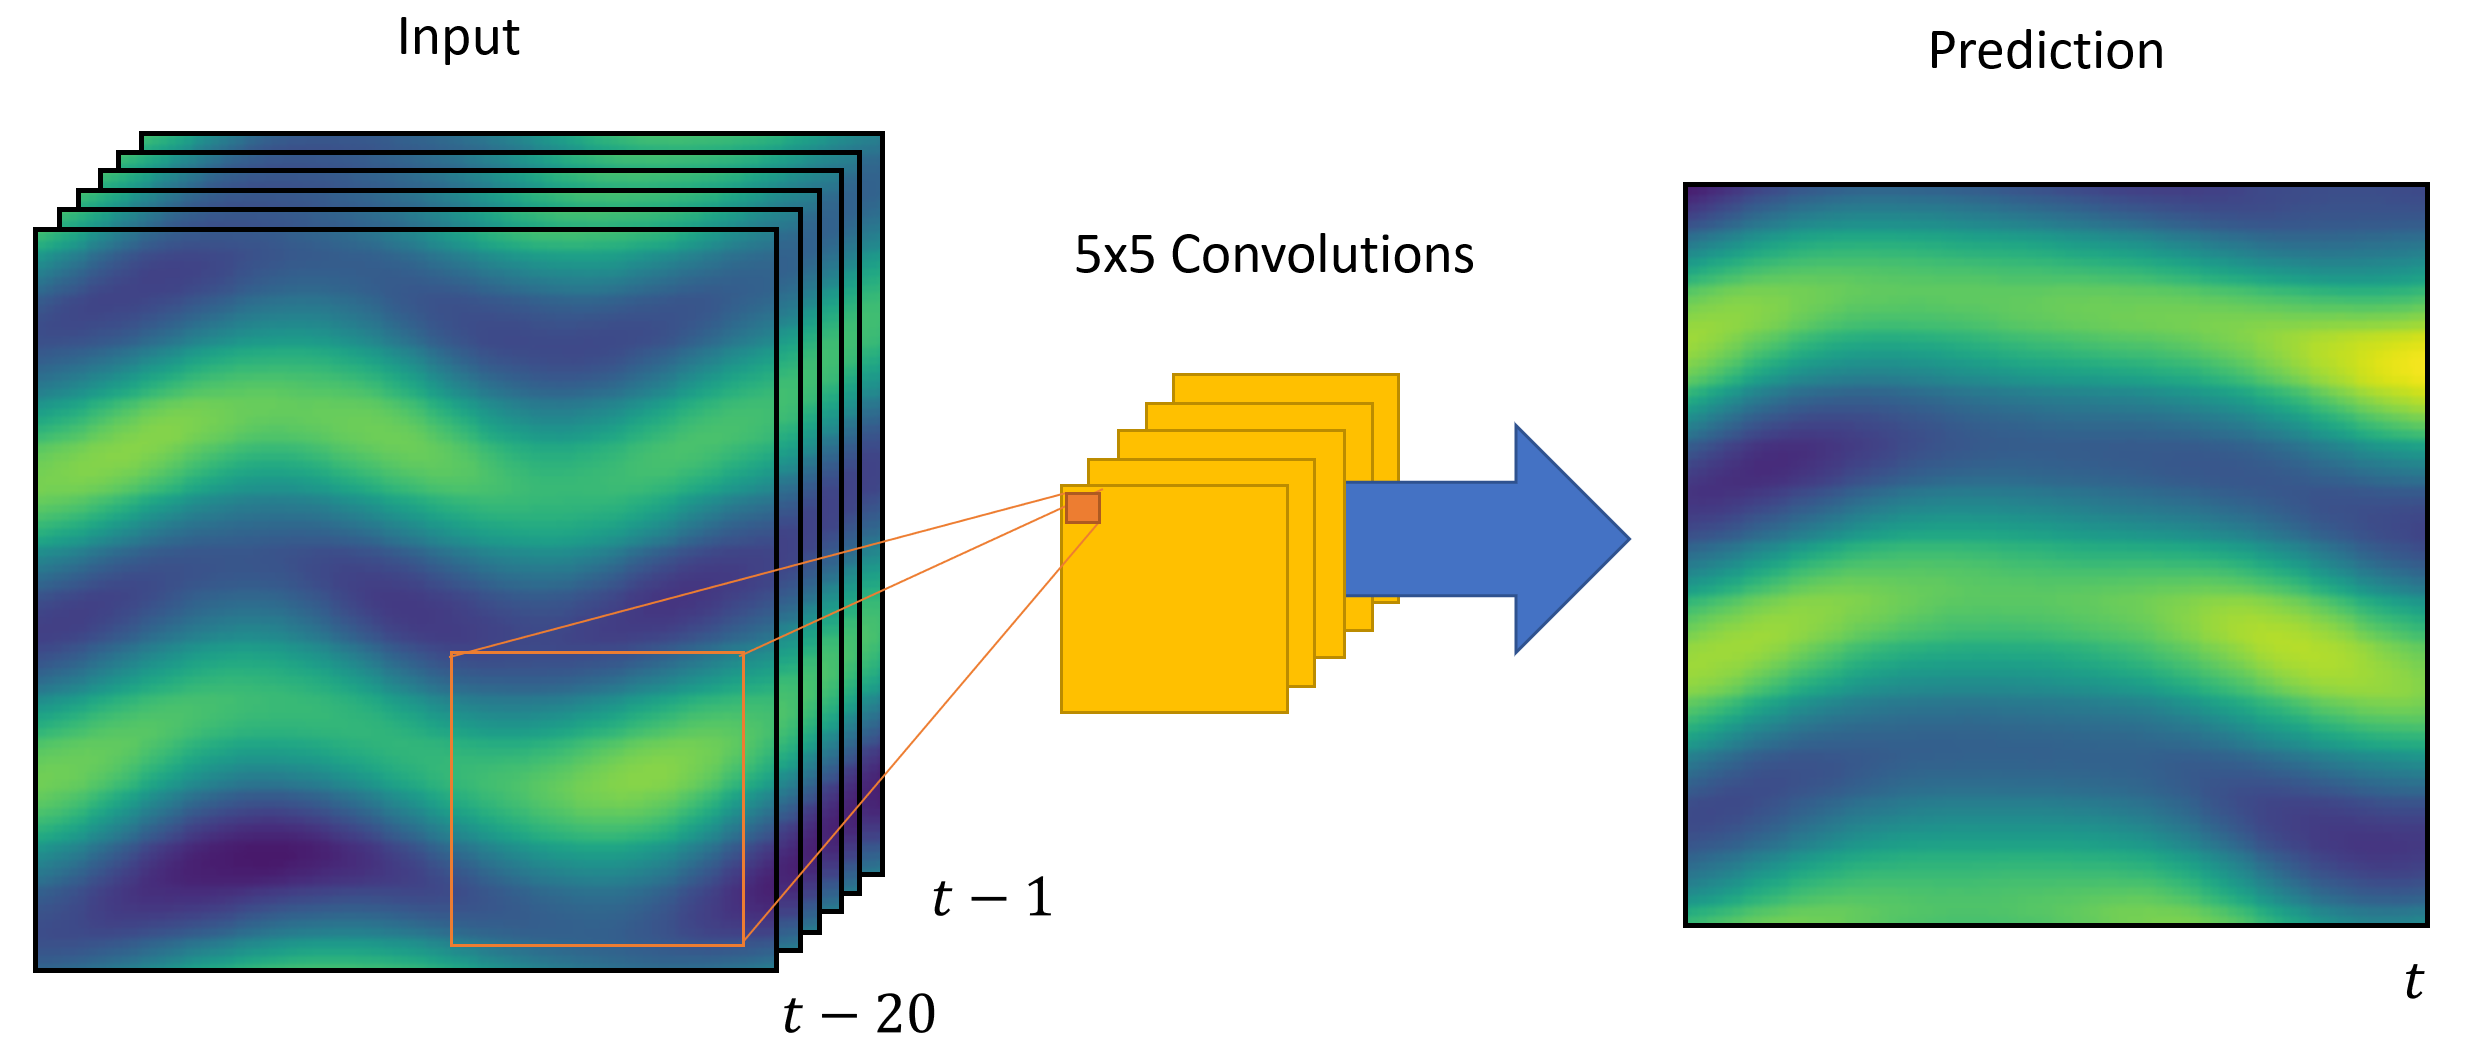
\includegraphics[width=0.7\textwidth]{images/setup.PNG}
		\caption{\small An single training example for predicting turbulent flow. Twenty frames of history are given at a single region of the turbulent flow and the network must predict the flow at the next time-step }
		\label{setup}
	\end{center}	
\end{figure}



\begin{figure}
	\begin{center}
		
\includegraphics[width=0.15\textwidth]{images/prediction/labe.png}
		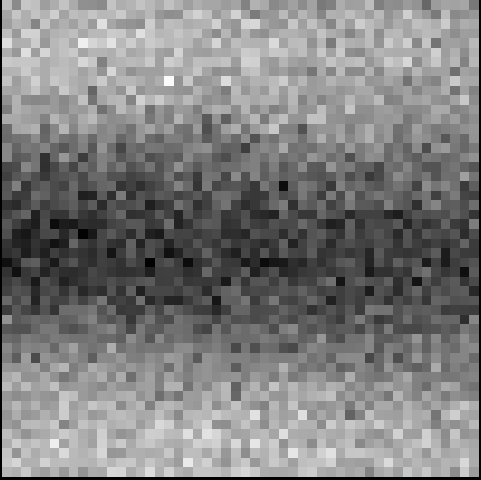
\includegraphics[width=0.15\textwidth]{images/prediction/5.png}
		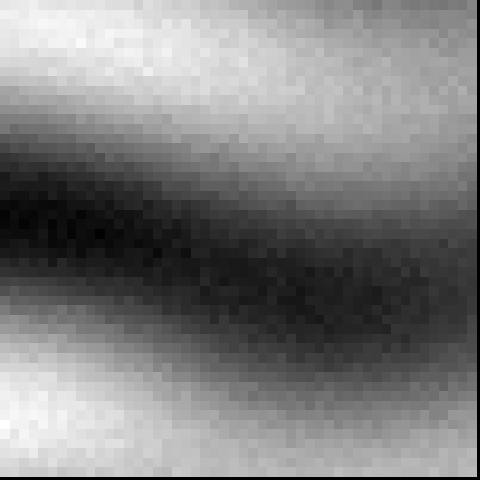
\includegraphics[width=0.15\textwidth]{images/prediction/10.png}
		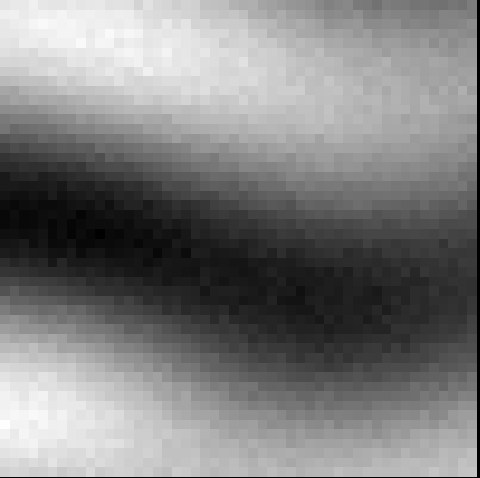
\includegraphics[width=0.15\textwidth]{images/prediction/15.png}
		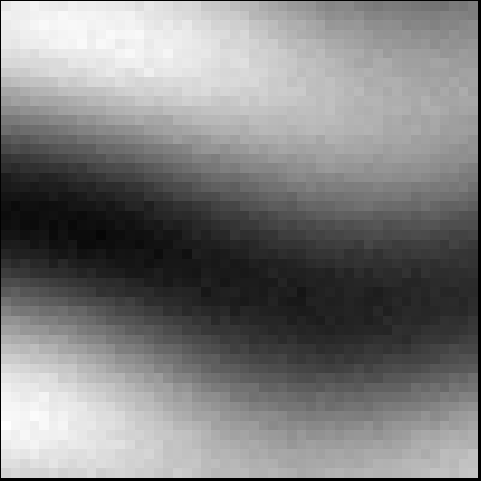
\includegraphics[width=0.15\textwidth]{images/prediction/20.png}
		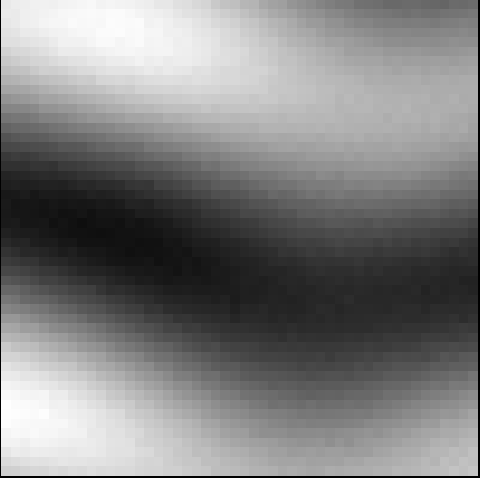
\includegraphics[width=0.15\textwidth]{images/prediction/25.png}
		\caption{\small (Left) Ground truth validation section of turbulent flow. (Remaining) Prediction of turbulent flow over, \num{1e+8}, \num{2e+8}, \num{3e+8}, \num{4e+8}, \num{5e+8} training batches respectively. Despite not occurring in the training set, the network is able to predict turbulent flow well across a single future time-step.}
		\label{mean_error}
	\end{center}	
\end{figure}

\begin{figure}
	\begin{center}
		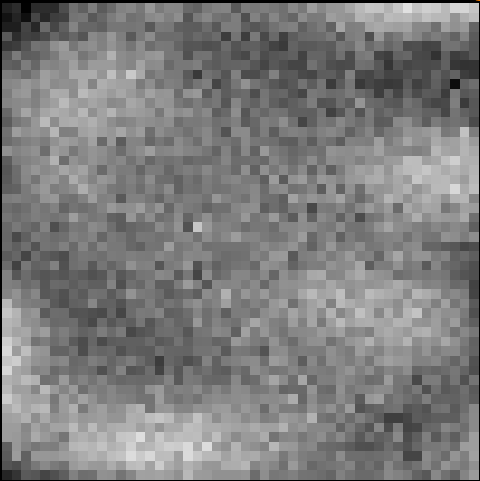
\includegraphics[width=0.39\textwidth]{images/mean_error_turbulence.png}
		\caption{\small Mean relative prediction error over 100  }
		\label{mean_error}
	\end{center}	
\end{figure}



In this period we developed deep networks capable of predicting turbulence over a 2D  flow generated in a shallow electrolyte layer. These networks predict the  well using only a single convolution over the history to reduce the latent embedding to 125 variables (5 features over 5x5 grid) see \ref{setup} for more information. Additionally we see that the prediction error is not strongly correlated with the edge of the image patch, which we would observe if the network was simply using local features. This suggests that the network has learned some non-local features over the entire turbulence trajectory.

Training uses 5000 patches (50 x 50 X 21) with 500 patches reserved for validation. The network uses a 5, 10px x 10px filters with a stride of 5 meaning a 50px x 50px x 20 time-step image is reduced to 5 activations in each of 5x5 grid locations. This is then fed to a fully connected layer and re-shaped to be 50x50, the shape of the next image for prediction. This network is then trained for 500,000,000 batches and achieves a validation accuracy of 0.001 MSE.



\end{document}